\documentclass[aspectratio=169]{beamer}

% Theme and Color Setup
\usetheme{Madrid}
\usecolortheme{whale}
\useinnertheme{rectangles}
\useoutertheme{miniframes}

% Additional Packages
\usepackage[utf8]{inputenc}
\usepackage[T1]{fontenc}
\usepackage{graphicx}
\usepackage{booktabs}
\usepackage{listings}
\usepackage{amsmath}
\usepackage{amssymb}
\usepackage{xcolor}
\usepackage{tikz}
\usepackage{pgfplots}
\pgfplotsset{compat=1.18}
\usetikzlibrary{positioning}
\usepackage{hyperref}

% Custom Colors
\definecolor{myblue}{RGB}{31, 73, 125}
\definecolor{mygray}{RGB}{100, 100, 100}
\definecolor{mygreen}{RGB}{0, 128, 0}
\definecolor{myorange}{RGB}{230, 126, 34}
\definecolor{mycodebackground}{RGB}{245, 245, 245}

% Set Theme Colors
\setbeamercolor{structure}{fg=myblue}
\setbeamercolor{frametitle}{fg=white, bg=myblue}
\setbeamercolor{title}{fg=myblue}
\setbeamercolor{section in toc}{fg=myblue}
\setbeamercolor{item projected}{fg=white, bg=myblue}
\setbeamercolor{block title}{bg=myblue!20, fg=myblue}
\setbeamercolor{block body}{bg=myblue!10}
\setbeamercolor{alerted text}{fg=myorange}

% Set Fonts
\setbeamerfont{title}{size=\Large, series=\bfseries}
\setbeamerfont{frametitle}{size=\large, series=\bfseries}
\setbeamerfont{caption}{size=\small}
\setbeamerfont{footnote}{size=\tiny}

% Document Start
\begin{document}

\frame{\titlepage}

\begin{frame}[fragile]
    \maketitle
\end{frame}

\begin{frame}[fragile]
    \frametitle{Introduction to Deep Reinforcement Learning - Overview}
    
    \begin{block}{Overview}
        Deep Reinforcement Learning (DRL) is a subfield of AI that integrates reinforcement learning and deep learning. It enables agents to learn optimal actions through interactions with their environment using trial and error.
    \end{block}

\end{frame}

\begin{frame}[fragile]
    \frametitle{Key Concepts in DRL}
    
    \begin{enumerate}
        \item \textbf{Reinforcement Learning Basics}:
        \begin{itemize}
            \item \textbf{Agent}: The decision-maker.
            \item \textbf{Environment}: The system with which the agent interacts.
            \item \textbf{State (s)}: Representation of the environment.
            \item \textbf{Action (a)}: Decisions available to the agent.
            \item \textbf{Reward (r)}: Feedback after an action.
        \end{itemize}
        
        \item \textbf{Deep Learning}:
        \begin{itemize}
            \item Utilizes neural networks to learn from large datasets.
            \item In DRL, these networks approximate functions to determine the best actions.
        \end{itemize}
    \end{enumerate}

\end{frame}

\begin{frame}[fragile]
    \frametitle{Significance of DRL in AI}
    
    \begin{itemize}
        \item \textbf{Complex Decision-Making}: DRL addresses high-dimensional state spaces effectively.
        \item \textbf{Real-World Applications}:
        \begin{itemize}
            \item \textbf{Gaming}: Superhuman strategies in games (e.g., AlphaGo).
            \item \textbf{Robotics}: Teaching robots through trial and error.
            \item \textbf{Finance}: Optimizing trading strategies with continuous learning.
        \end{itemize}
    \end{itemize}
    
\end{frame}

\begin{frame}[fragile]
    \frametitle{Examples of DRL}
    
    \begin{itemize}
        \item \textbf{AlphaGo}:
        \begin{itemize}
            \item Used DRL to master the game of Go.
            \item Demonstrated AI's capability in complex strategic tasks.
        \end{itemize}
        
        \item \textbf{Self-Driving Cars}:
        \begin{itemize}
            \item Employ DRL for navigation and obstacle avoidance.
            \item Continuously learn from driving data.
        \end{itemize}
    \end{itemize}

\end{frame}

\begin{frame}[fragile]
    \frametitle{Key Points to Emphasize}
    
    \begin{itemize}
        \item \textbf{Combines Strengths}: Merges exploration-exploitation in RL with function approximation of deep learning.
        \item \textbf{Learning Paradigms}:
        \begin{itemize}
            \item \textbf{Exploration}: Trying new actions to discover outcomes.
            \item \textbf{Exploitation}: Choosing known actions for maximum reward.
        \end{itemize}
    \end{itemize}
    
\end{frame}

\begin{frame}[fragile]
    \frametitle{Mathematical Formulation}
    
    To illustrate how agents learn, consider the \textbf{Q-Learning Update Rule}:
    
    \begin{equation}
    Q(s, a) \leftarrow Q(s, a) + \alpha \left[ r + \gamma \max_a Q(s', a) - Q(s, a) \right]
    \end{equation}
    
    \begin{itemize}
        \item \textbf{Q(s, a)}: Expected future reward for action \(a\) in state \(s\).
        \item \(\alpha\): Learning rate.
        \item \(\gamma\): Discount factor for future rewards.
        \item \(s'\): New state following action \(a\).
    \end{itemize}
    
\end{frame}

\begin{frame}[fragile]
    \frametitle{Conclusion}
    
    Deep Reinforcement Learning is a powerful tool in AI, capable of addressing complex sequential decision-making challenges. By utilizing deep neural networks, DRL scales effectively in intricate environments, thereby advancing the frontiers of what AI can achieve.
    
\end{frame}

\begin{frame}[fragile]
    \frametitle{Foundations of Reinforcement Learning - Learning Objectives}
    \begin{enumerate}
        \item Understand core components of reinforcement learning (RL): agents, environments, rewards, and policies.
        \item Recognize how these components interact to inform decision-making in machine learning.
    \end{enumerate}
\end{frame}

\begin{frame}[fragile]
    \frametitle{Foundations of Reinforcement Learning - Key Concepts}
    \begin{block}{1. Agents}
        \begin{itemize}
            \item \textbf{Definition:} An agent is an entity that makes observations and takes actions within an environment.
            \item \textbf{Example:} A robot navigating a maze decides which direction to move based on its observations.
        \end{itemize}
    \end{block}

    \begin{block}{2. Environments}
        \begin{itemize}
            \item \textbf{Definition:} The environment is everything that an agent interacts with, providing feedback based on actions.
            \item \textbf{Example:} The maze with walls, pathways, and obstacles that the agent must navigate.
        \end{itemize}
    \end{block}
\end{frame}

\begin{frame}[fragile]
    \frametitle{Foundations of Reinforcement Learning - Key Concepts (cont.)}
    \begin{block}{3. Rewards}
        \begin{itemize}
            \item \textbf{Definition:} A reward is a scalar feedback signal the agent receives after performing an action.
            \item \textbf{Example:} Reaching the exit of the maze gives a +10 reward, hitting a wall incurs -5.
        \end{itemize}
    \end{block}

    \begin{block}{4. Policies}
        \begin{itemize}
            \item \textbf{Definition:} A policy defines the agent's behavior at any time, mapping situations to actions.
            \item \textbf{Example:} A policy could be "always turn left," or a more complex policy based on various observations.
        \end{itemize}
    \end{block}
\end{frame}

\begin{frame}[fragile]
    \frametitle{Interaction Between Components}
    \begin{block}{Feedback Loop}
        \begin{itemize}
            \item The \textbf{agent} observes the \textbf{environment}, takes an \textbf{action} based on its \textbf{policy}, and receives a \textbf{reward}.
            \item \textbf{Cycle:}
            \begin{enumerate}
                \item Observe State
                \item Select Action
                \item Receive Reward
                \item Update Policy
            \end{enumerate}
        \end{itemize}
    \end{block}
\end{frame}

\begin{frame}[fragile]
    \frametitle{Key Points and Code Snippet Example}
    \begin{itemize}
        \item The relationship between these components forms the backbone of reinforcement learning systems.
        \item RL learns through trial-and-error, differing from supervised learning.
        \item The ultimate goal is to learn an optimal policy that maximizes cumulative rewards.
    \end{itemize}

    \begin{lstlisting}[language=python]
initialize agent
initialize environment

for episode in range(num_episodes):
    state = environment.reset()
    done = False
    while not done:
        action = agent.select_action(state)
        next_state, reward, done = environment.step(action)
        agent.update_policy(state, action, reward, next_state)
        state = next_state
    \end{lstlisting}
\end{frame}

\begin{frame}[fragile]
    \frametitle{Markov Decision Processes (MDPs) - Introduction}
    \begin{block}{Introduction to MDPs}
        Markov Decision Processes (MDPs) provide a mathematical framework for modeling decision-making situations where outcomes are partly random and partly under the control of a decision-maker (agent).
        MDPs are fundamental to reinforcement learning and help in optimizing decisions to achieve maximum cumulative rewards.
    \end{block}
\end{frame}

\begin{frame}[fragile]
    \frametitle{Markov Decision Processes (MDPs) - Key Components}
    An MDP is defined by the following components:
    \begin{enumerate}
        \item \textbf{States (S)}: A set of states that represents all possible situations the agent could find itself in.
        \begin{itemize}
            \item Example: In a chess game, each unique arrangement of pieces can be considered a different state.
        \end{itemize}
        
        \item \textbf{Actions (A)}: A set of actions available to the agent in each state.
        \begin{itemize}
            \item Example: In chess, actions might include moving a pawn, queen, or any other piece.
        \end{itemize}
        
        \item \textbf{Transition Function (T)}: A probability function that defines the dynamics of the system.
        \begin{itemize}
            \item Notation: $T(s, a, s')$ is the probability of transitioning to state $s'$ from state $s$ after taking action $a$.
        \end{itemize}
        
        \item \textbf{Rewards (R)}: A reward function assigning a numerical value for transitioning between states given a specific action.
        \begin{itemize}
            \item Notation: $R(s, a, s')$ represents the expected reward received after transitioning from state $s$ to state $s'$ due to action $a$.
        \end{itemize}
        
        \item \textbf{Policy ($\pi$)}: A strategy that defines how to choose actions based on the current state.
        \begin{itemize}
            \item Example: A policy could be deterministic or stochastic.
        \end{itemize}
    \end{enumerate}
\end{frame}

\begin{frame}[fragile]
    \frametitle{Markov Decision Processes (MDPs) - Characteristics and Applications}
    
    \begin{block}{Characteristics}
        \begin{itemize}
            \item \textbf{Markov Property}: MDPs assume that the future state is only influenced by the present state, simplifying decision-making modeling.
        \end{itemize}
    \end{block}

    \begin{block}{Visual Description of MDP}
        Consider a grid-world environment:
        \begin{center}
            \begin{verbatim}
            +---+---+---+
            | S | R | G |
            +---+---+---+
            |   |   |   |
            +---+---+---+
            |   |   |   |
            +---+---+---+
            \end{verbatim}
        \end{center}
        Where:
        \begin{itemize}
            \item S = Start state
            \item R = Reward cell
            \item G = Goal cell
        \end{itemize}
    \end{block}

    \begin{block}{Key Points to Emphasize}
        \begin{itemize}
            \item MDPs serve as a structured method to solve complex decision-making problems.
            \item They facilitate algorithms such as Value Iteration and Policy Iteration.
            \item Applications include robotics, finance, and healthcare decision-making.
        \end{itemize}
    \end{block}
\end{frame}

\begin{frame}[fragile]
  \frametitle{Key Algorithms in Reinforcement Learning - Overview}
  \begin{itemize}
    \item Learning Objectives:
    \begin{itemize}
      \item Understand the distinctions between value-based and policy-based methods.
      \item Explore key algorithms: Q-learning (value-based) and Policy Gradient methods (policy-based).
    \end{itemize}
  \end{itemize}
\end{frame}

\begin{frame}[fragile]
  \frametitle{Key Algorithms in Reinforcement Learning - Value-Based Methods}
  \begin{block}{Value-Based Methods}
    Value-based methods focus on estimating the value of actions taken in specific states, deriving policies indirectly from these estimates.
  \end{block}

  \begin{block}{Q-Learning}
    \begin{itemize}
      \item \textbf{Definition}: An off-policy algorithm learning the value of actions with Q-values.
      \item \textbf{Formula}:
      \[
      Q(s, a) \leftarrow Q(s, a) + \alpha \left( r + \gamma \max_{a'} Q(s', a') - Q(s, a) \right)
      \]
      \begin{itemize}
        \item \( Q(s, a) \): Current estimated Q-value of action \( a \) in state \( s \)
        \item \( \alpha \): Learning rate (0 < \( \alpha \) ≤ 1)
        \item \( r \): Reward received
        \item \( \gamma \): Discount factor (0 ≤ \( \gamma \) < 1)
        \item \( s' \): Next state
      \end{itemize}
      \item \textbf{Example}: Chess board configurations to estimate optimal moves based on past experiences.
    \end{itemize}
  \end{block}
\end{frame}

\begin{frame}[fragile]
  \frametitle{Key Algorithms in Reinforcement Learning - Policy-Based Methods}
  \begin{block}{Policy-Based Methods}
    Policy-based methods directly optimize the policy using gradient ascent techniques.
  \end{block}

  \begin{block}{Policy Gradient Methods}
    \begin{itemize}
      \item \textbf{Definition}: Adjust policy parameters directly, estimating the gradient of expected reward.
      \item \textbf{Objective}:
      \[
      J(\theta) = \mathbb{E}_{\tau \sim \pi_\theta} \left[ \sum_{t=0}^{T} r_t \right]
      \]
      \item \textbf{Update Rule}:
      \[
      \theta \leftarrow \theta + \alpha \nabla J(\theta)
      \]
      \begin{itemize}
        \item \( \theta \): Parameters of the policy
        \item \( \nabla J(\theta) \): Gradient of expected reward with respect to \( \theta \)
      \end{itemize}
      \item \textbf{Example}: Robotic arm control, optimizing joint angles to maximize reach based on performance feedback.
    \end{itemize}
  \end{block}

  \begin{block}{Key Points}
    \begin{itemize}
      \item Useful for high-dimensional, continuous action spaces.
      \item Prone to higher variance; reduction techniques (e.g., baselines) help stabilize training.
    \end{itemize}
  \end{block}
\end{frame}

\begin{frame}[fragile]
  \frametitle{Key Algorithms in Reinforcement Learning - Summary}
  \begin{itemize}
    \item \textbf{Value-Based}: Q-learning quantifies action values and derives a policy.
    \item \textbf{Policy-Based}: Policy gradients optimize the action selection policy through gradients.
  \end{itemize}

  \begin{block}{Conclusion}
    Understanding both approaches equips us to tackle various reinforcement learning problems effectively, allowing for adaptive exploration and exploitation of environments.
  \end{block}
\end{frame}

\begin{frame}[fragile]
    \frametitle{Introduction to Deep Learning}
    \begin{block}{Overview of Deep Learning}
        Deep learning is a subset of machine learning utilizing artificial neural networks to understand complex patterns in high-dimensional data. Inspired by the human brain's structure and function.
    \end{block}
\end{frame}

\begin{frame}[fragile]
    \frametitle{Core Principles of Deep Learning}
    \begin{itemize}
        \item \textbf{Neural Networks:} Layers of interconnected nodes (neurons) with weights adjusted during training.
        \item \textbf{Backpropagation:} Learning process that calculates gradients to minimize the error between predicted and actual outcomes.
    \end{itemize}
\end{frame}

\begin{frame}[fragile]
    \frametitle{Key Characteristics}
    \begin{itemize}
        \item \textbf{Hierarchical Feature Learning:} Automatically extracts features in a hierarchy from raw data (e.g., pixels in images, words in text).
        \item \textbf{Scalability:} Handles large volumes of data, improving performance as more data becomes available.
        \item \textbf{Representation Learning:} Learns significant and hidden patterns automatically, reducing the need for manual feature engineering.
    \end{itemize}
\end{frame}

\begin{frame}[fragile]
    \frametitle{Integration with Reinforcement Learning}
    \begin{block}{Reinforcement Learning (RL) Paradigm}
        In RL, agents learn from consequences of their actions through trial and error to maximize cumulative rewards.
    \end{block}
    
    \begin{itemize}
        \item \textbf{Why Combine Deep Learning with RL?}
            \begin{itemize}
                \item Handles high-dimensional spaces efficiently.
                \item Improved function approximation, allowing complex environments to be learned from experience.
            \end{itemize}
    \end{itemize}
\end{frame}

\begin{frame}[fragile]
    \frametitle{Example: AlphaGo}
    \begin{itemize}
        \item \textbf{Game:} Go, a board game with an immensely large state space.
        \item \textbf{Deep Learning Role:} Neural networks evaluate board positions.
        \item \textbf{Reinforcement Learning Role:} The system learns by playing millions of games against itself, refining strategies based on outcomes.
    \end{itemize}
\end{frame}

\begin{frame}[fragile]
    \frametitle{Conclusion}
    \begin{block}{Key Points to Emphasize}
        \begin{itemize}
            \item \textbf{Transformative Potential:} Deep reinforcement learning advances AI in various fields, from gaming to robotics.
            \item \textbf{Interdisciplinary Nature:} Combines concepts from computer science, operational research, and neuroscience.
        \end{itemize}
    \end{block}
    \begin{block}{Next Steps}
        Explore how the architecture of Deep Q-Networks (DQN) illustrates the synergy of deep learning and reinforcement learning in the following slide.
    \end{block}
\end{frame}

\begin{frame}[fragile]
  \frametitle{Deep Q-Networks (DQN)}
  
  \begin{block}{Learning Objectives}
    \begin{itemize}
      \item Understand the architecture of Deep Q-Networks (DQN).
      \item Explore how DQNs integrate deep learning with reinforcement learning.
      \item Identify the benefits of using neural networks in Q-learning.
    \end{itemize}
  \end{block}
\end{frame}

\begin{frame}[fragile]
  \frametitle{Introduction to DQNs}
  
  Deep Q-Networks (DQN) is a groundbreaking approach that combines the principles of 
  \textbf{Deep Learning} and \textbf{Reinforcement Learning (RL)}. 
  DQNs leverage neural networks to approximate the Q-value function, allowing agents to learn 
  effective policies in complex environments.
\end{frame}

\begin{frame}[fragile]
  \frametitle{DQN Architecture}
  
  \begin{itemize}
    \item \textbf{Core Components:}
      \begin{itemize}
        \item \textbf{Input Layer:} Receives the state representation of the environment (e.g., pixel data from a video game).
        \item \textbf{Hidden Layers:} Multiple layers of neurons with nonlinear activations (e.g., ReLU).
        \item \textbf{Output Layer:} Outputs Q-values for each possible action in the given state.
      \end{itemize}
    
    \item \textbf{Mathematical Representation:}
      \begin{equation}
        Q(s, a; \theta) = \text{NeuralNet}(s; \theta)
      \end{equation}
      where:
      \begin{itemize}
        \item $s$ = current state
        \item $a$ = action taken
        \item $\theta$ = weights of the neural network
      \end{itemize}
  \end{itemize}
\end{frame}

\begin{frame}[fragile]
  \frametitle{Combining Deep Learning with RL}
  
  \begin{itemize}
    \item \textbf{Function Approximation:} 
      DQNs use a neural network to approximate Q-values instead of a lookup table, enabling:
      \begin{itemize}
        \item Handling large state spaces (e.g., pixels in an image).
        \item Generalization across similar states.
      \end{itemize}
    
    \item \textbf{Experience Replay:} 
      DQNs use a replay buffer to enhance learning efficiency:
      \begin{itemize}
        \item Store experiences (state, action, reward, next state).
        \item Randomly sample mini-batches to update the network, stabilizing training.
      \end{itemize}
  \end{itemize}
\end{frame}

\begin{frame}[fragile]
  \frametitle{Key Points to Emphasize}
  
  \begin{itemize}
    \item \textbf{Dynamic Learning:} DQNs adjust policies via Q-learning while utilizing a deep learning model.
    \item \textbf{Handling Complexity:} Effective in complex environments like video games (e.g., Atari).
    \item \textbf{Stability Improvements:} Techniques such as fixed Q-targets and experience replay enhance stability.
  \end{itemize}
\end{frame}

\begin{frame}[fragile]
  \frametitle{Example Illustration}
  
  Imagine a DQN agent playing a video game:
  \begin{itemize}
    \item The input could be the game screen (state representation).
    \item Hidden layers process this data to evaluate actions (e.g., jump, move left, shoot) based on past experiences.
    \item The agent maximizes its score by adjusting its policy using stored experiences.
  \end{itemize}
\end{frame}

\begin{frame}[fragile]
  \frametitle{DQN Pseudocode}
  
  \begin{lstlisting}[language=python]
Initialize replay buffer D
Initialize action-value function Q with random weights
For episode = 1 to M do:
    Initialize state s
    For t = 1 to T do:
        Choose action a using ε-greedy policy based on Q
        Perform action a, observe reward r and new state s'
        Store transition (s, a, r, s') in D
        Sample a random mini-batch from D
        Update Q by minimizing:
        ∑(r + γ max Q(s', a'; θ') - Q(s, a; θ))^2
        Update the target network periodically
  \end{lstlisting}
\end{frame}

\begin{frame}[fragile]
    \frametitle{Experience Replay - Overview}
    \begin{block}{What is Experience Replay?}
        Experience Replay is a technique in Deep Reinforcement Learning (DRL) that enhances training efficiency by storing agent experiences in a replay buffer. 
        This allows the agent to sample past experiences randomly, improving learning stability by breaking the correlation between consecutive experiences.
    \end{block}
\end{frame}

\begin{frame}[fragile]
    \frametitle{Experience Replay - How Does it Work?}
    \begin{enumerate}
        \item \textbf{Experience Buffer}: Stores tuples of state, action, reward, next state, and done flag: 
        \( (s_t, a_t, r_t, s_{t+1}, d_t) \).
        
        \item \textbf{Sampling}: During training, a mini-batch of experiences is sampled randomly to update the DQN. 
        This randomness helps prevent overfitting to recent experiences.
        
        \item \textbf{Training}: Updates Q-value estimates using the Bellman equation:
        \begin{equation}
            Q(s_t, a_t) \leftarrow r_t + \gamma \max_a Q(s_{t+1}, a)
        \end{equation}
        where \( \gamma \) is the discount factor.
    \end{enumerate}
\end{frame}

\begin{frame}[fragile]
    \frametitle{Experience Replay - Importance and Example}
    \begin{block}{Importance in DQN}
        \begin{itemize}
            \item \textbf{Stabilizes Learning}: Uses a diverse set of past experiences.
            \item \textbf{Efficiency}: Reuses past experiences, which is more sample-efficient.
            \item \textbf{Less Correlation}: Random sampling breaks the sequential correlation in experiences.
        \end{itemize}
    \end{block}
    
    \begin{block}{Example Illustration}
        \textbf{Scenario}: An agent navigates a maze:
        \begin{itemize}
            \item Movement from state \( s_1 \) to \( s_2 \) with reward \( r_1 \).
            \item Movement from \( s_2 \) to \( s_3 \) with reward \( r_2 \).
        \end{itemize}
        Experiences stored: \( (s_1, a_1, r_1, s_2, d_1) \) and \( (s_2, a_2, r_2, s_3, d_2) \).
    \end{block}
\end{frame}

\begin{frame}[fragile]
    \frametitle{Target Network in Deep Q-Networks (DQNs)}
    \begin{block}{What is a Target Network?}
        A \textbf{Target Network} is a duplicate of the Q-network used in DQNs that stabilizes training by being updated less frequently.
    \end{block}
\end{frame}

\begin{frame}[fragile]
    \frametitle{Target Network: Purpose}
    \begin{itemize}
        \item \textbf{Stabilization of Training:}
            \begin{itemize}
                \item Reduces oscillation in Q-values during training.
                \item Provides a consistent target, updated periodically.
            \end{itemize}
        \item \textbf{Breaking Correlation:}
            \begin{itemize}
                \item Separates updates of primary Q-network and target network.
                \item Helps converge learning by breaking feedback loops.
            \end{itemize}
    \end{itemize}
\end{frame}

\begin{frame}[fragile]
    \frametitle{How Does the Target Network Work?}
    \begin{block}{Architecture}
        The DQN consists of two networks: the primary Q-network (online) and the target network, initially identical.
    \end{block}
    
    \begin{block}{Soft Update Mechanism}
        \begin{equation}
        Q_{\text{target}} = \tau \cdot Q_{\text{online}} + (1 - \tau) \cdot Q_{\text{target}}
        \end{equation}
        where $\tau$ is a small value determining the update frequency (e.g., 0.1).
    \end{block}

    \begin{itemize}
        \item Use the target network for target calculation:
        \begin{equation}
        Y = r + \gamma \max Q_{\text{target}}(s', a')
        \end{equation}
        \item Loss function for updating primary Q-network:
        \begin{equation}
        \text{Loss} = \left( Y - Q_{\text{online}}(s, a) \right)^2
        \end{equation}
    \end{itemize}
\end{frame}

\begin{frame}[fragile]
    \frametitle{Actor-Critic Methods - Overview}
    \begin{block}{Overview of Actor-Critic Architecture}
        \begin{itemize}
            \item \textbf{Actor:} Selects actions using a policy ($\pi$) that maps states to action probabilities.
            \item \textbf{Critic:} Evaluates the actions by providing a value function ($V$) that estimates expected future rewards.
        \end{itemize}
    \end{block}
    
    \begin{block}{How They Work Together}
        \begin{itemize}
            \item The actor proposes actions, while the critic evaluates them, allowing for iterative improvement:
                \begin{itemize}
                    \item The \textbf{actor} improves its policy based on critics' feedback.
                    \item The \textbf{critic} refines its value estimations for accurate evaluations.
                \end{itemize}
        \end{itemize}
    \end{block}
    
    \begin{block}{Diagram}
        \includegraphics[width=0.7\textwidth]{actor_critic_diagram.png} % Placeholder for diagram
    \end{block}
\end{frame}

\begin{frame}[fragile]
    \frametitle{Actor-Critic Methods - Advantages}
    \begin{block}{Advantages of Actor-Critic Methods}
        \begin{itemize}
            \item \textbf{Stability and Efficiency}: Separation of policy and value function leads to greater stability during training.
            \item \textbf{Continuous Action Spaces}: Effective in environments requiring continuous actions.
            \item \textbf{Sample Efficiency}: Learns from fewer samples by utilizing both action-value and state-value functions.
            \item \textbf{Flexibility}: Adapts to various value estimation forms (e.g., Temporal Difference Learning) and policies (deterministic or stochastic).
        \end{itemize}
    \end{block}
\end{frame}

\begin{frame}[fragile]
    \frametitle{Actor-Critic Methods - Application and Conclusion}
    \begin{block}{Example: Application in Robotics}
        Consider an autonomous robot navigating through obstacles:
        \begin{itemize}
            \item \textbf{Actor:} Learns to choose movements (left, right, forward, backward) based on position and obstacle proximity.
            \item \textbf{Critic:} Evaluates movements by estimating expected future rewards based on reaching a target while avoiding obstacles.
        \end{itemize}
    \end{block}
    
    \begin{block}{Key Points to Emphasize}
        \begin{itemize}
            \item Combines advantages of policy-based and value-based methods.
            \item Effective in complex action spaces.
            \item Enables convergent learning and robust policy development.
        \end{itemize}
    \end{block}

    \begin{block}{Conclusion}
        Actor-critic methods are powerful in deep reinforcement learning, enhancing efficiency, stability, and adaptability in complex environments.
    \end{block}
\end{frame}

\begin{frame}[fragile]
  \frametitle{Proximal Policy Optimization (PPO) - Introduction}
  Proximal Policy Optimization (PPO) is a widely used algorithm in deep reinforcement learning, specifically in actor-critic methods. 
  It addresses some limitations of earlier algorithms while maintaining simplicity and solid performance.

  \begin{itemize}
    \item \textbf{Actor-Critic Architecture:}
      \begin{itemize}
        \item \textbf{Actor:} Decides which action to take based on the current state.
        \item \textbf{Critic:} Evaluates actions by computing the value function.
      \end{itemize}
    
    \item \textbf{Policy Gradient Approach:} 
      PPO directly optimizes the policy instead of deriving it from the value function.
  \end{itemize}
\end{frame}

\begin{frame}[fragile]
  \frametitle{PPO - Key Features and Improvements}
  
  \begin{enumerate}
    \item \textbf{Clipped Objective Function:} 
      \begin{itemize}
        \item Ensures policy updates do not deviate significantly from the previous policy, minimizing the chance of performance collapse.
        \item Objective function:
        \begin{equation}
          L(\theta) = \mathbb{E}_t \left[ \min\left(\frac{\pi_\theta(a_t|s_t)}{\pi_{\theta_{old}}(a_t|s_t)} \hat{A}_t, g(\epsilon, \hat{A}_t)\right)\right]
        \end{equation}
        where:
        \begin{itemize}
          \item \( \hat{A}_t \) = Advantage estimate at time \( t \)
          \item \( g(\epsilon, \hat{A}_t) = (1 + \epsilon) \hat{A}_t \) if \( \hat{A}_t \geq 0 \), else \( (1 - \epsilon) \hat{A}_t \)
        \end{itemize}
      \end{itemize}
    
    \item \textbf{Multiple Epochs:} 
      \begin{itemize}
        \item Allows multiple updates per batch, leading to more stable learning and better sample efficiency.
      \end{itemize}
    
    \item \textbf{Mini-batch Optimization:} 
      \begin{itemize}
        \item Splits data into smaller batches for multiple updates within the same learning step, enhancing computational efficiency and stability.
      \end{itemize}
  \end{enumerate}
\end{frame}

\begin{frame}[fragile]
  \frametitle{Example Scenario and Summary}
  
  \textbf{Example Scenario:} 
  Consider a robotic arm trained using PPO to manipulate objects. The actor decides the next movement based on its current state (e.g., arm position), while the critic evaluates how good that movement is based on the achieved reward (e.g., correctly picking up an object). 

  \bigskip
  
  \textbf{Summary and Key Points:} 
  \begin{itemize}
    \item PPO is robust, effective, and widely used in reinforcement learning.
    \item Advantages include simplicity, stability through clipped updates, and effective sample usage via mini-batching and multiple epochs.
    \item Its ease of implementation and strong empirical performance make it popular across various applications in deep reinforcement learning.
  \end{itemize}
\end{frame}

\begin{frame}[fragile]
    \frametitle{Applications of Deep Reinforcement Learning}
    \begin{block}{Learning Objectives}
        \begin{itemize}
            \item Understand key domains where deep reinforcement learning (DRL) is applied.
            \item Recognize specific applications and their implications in real-world scenarios.
        \end{itemize}
    \end{block}
\end{frame}

\begin{frame}[fragile]
    \frametitle{Overview}
    Deep Reinforcement Learning combines reinforcement learning (RL) principles with deep learning techniques, 
    enabling machines to make decisions based on high-dimensional sensory inputs. Its applicability spans various fields, 
    each utilizing DRL's ability to learn optimal policies through trial and error.
\end{frame}

\begin{frame}[fragile]
    \frametitle{Key Applications - Part 1}
    \begin{enumerate}
        \item \textbf{Gaming:}
            \begin{itemize}
                \item \textbf{Examples:} AlphaGo and OpenAI Five
                \item \textbf{AlphaGo:} Defeated world champion Go player by learning from millions of games with deep neural networks and Monte Carlo Tree Search.
                \item \textbf{OpenAI Five:} Played Dota 2, coordinating with teammates and strategizing effectively against human opponents.
                \item \textbf{Key Point:} DRL excels in environments with clear reward signals and can achieve superhuman performance in strategic decision-making.
            \end{itemize}
        
        \item \textbf{Robotics:}
            \begin{itemize}
                \item \textbf{Examples:} Autonomous Navigation and Manipulation
                \item Robots learn to walk, pick, and place objects, improving precision through simulation feedback.
                \item \textbf{Key Point:} DRL enables robots to learn from experience, adapting with minimal programming intervention.
            \end{itemize}
    \end{enumerate}
\end{frame}

\begin{frame}[fragile]
    \frametitle{Key Applications - Part 2}
    \begin{enumerate}
        \setcounter{enumi}{2} % Continue the enumeration
        \item \textbf{Finance:}
            \begin{itemize}
                \item \textbf{Example:} Algorithmic Trading
                \item DRL constructs trading strategies by analyzing market conditions and optimizing portfolio management.
                \item \textbf{Key Point:} Continuous learning in DRL enables real-time decision making in dynamic market environments.
            \end{itemize}
        
        \item \textbf{Healthcare:}
            \begin{itemize}
                \item \textbf{Example:} Personalized Treatment Recommendations
                \item DRL assists in creating protocols considering patient history and treatment outcomes.
                \item \textbf{Key Point:} DRL optimizes complex decision processes in healthcare, enhancing patient care.
            \end{itemize}
    \end{enumerate}
\end{frame}

\begin{frame}[fragile]
    \frametitle{Key Applications - Part 3}
    \begin{itemize}
        \item \textbf{Transportation:}
            \begin{itemize}
                \item \textbf{Example:} Smart Traffic Management
                \item DRL optimizes traffic signals based on real-time conditions to reduce congestion.
                \item \textbf{Key Point:} DRL can dynamically adapt to changing environments, improving urban infrastructure efficiency.
            \end{itemize}
    \end{itemize}

    \begin{block}{Conclusion}
        Deep Reinforcement Learning solves complex decision-making tasks across diverse domains. By leveraging vast amounts of data and learning from experience, DRL shapes innovations crucial for technological advances and efficiency improvements.
    \end{block}
\end{frame}

\begin{frame}[fragile]
    \frametitle{References}
    \begin{itemize}
        \item DeepMind's Publications
        \item OpenAI Research
        \item Industry Applications in Robotics and Finance
    \end{itemize}
\end{frame}

\begin{frame}[fragile]
    \frametitle{Challenges in Deep Reinforcement Learning - Overview}
    \begin{block}{Overview}
        Deep Reinforcement Learning (DRL) combines reinforcement learning principles with deep learning architectures. While it has led to impressive advancements in various fields, it presents several challenges. Understanding these challenges is crucial for developing effective DRL systems.
    \end{block}
\end{frame}

\begin{frame}[fragile]
    \frametitle{Challenges in Deep Reinforcement Learning - Key Challenges}
    \begin{enumerate}
        \item \textbf{Sample Inefficiency}
        \item \textbf{Generalization}
        \item \textbf{Stability and Convergence}
        \item \textbf{Credit Assignment Problem}
    \end{enumerate}
\end{frame}

\begin{frame}[fragile]
    \frametitle{Sample Inefficiency}
    \begin{itemize}
        \item \textbf{Explanation}: Many DRL algorithms require a large number of interactions with the environment to learn effective policies, leading to high computational costs.
        \item \textbf{Example}: An agent may need to play thousands of games to learn optimal strategies.
        \item \textbf{Key Point}: Techniques like experience replay and more efficient exploration strategies can help mitigate this issue.
    \end{itemize}
\end{frame}

\begin{frame}[fragile]
    \frametitle{Generalization}
    \begin{itemize}
        \item \textbf{Explanation}: DRL agents often overfit training environments and struggle to generalize to new situations.
        \item \textbf{Example}: An agent trained in a specific maze may falter when presented with minor layout variations.
        \item \textbf{Key Point}: Regularization techniques, domain randomization, and exposure to diverse scenarios can enhance generalization.
    \end{itemize}
\end{frame}

\begin{frame}[fragile]
    \frametitle{Stability and Convergence}
    \begin{itemize}
        \item \textbf{Explanation}: Sensitivity to hyperparameters can lead to unstable training processes and inconsistent performance.
        \item \textbf{Example}: In training a robot to balance on two legs, changes in learning rates can derail convergence.
        \item \textbf{Key Point}: Techniques such as target networks and normalized rewards can improve overall stability.
    \end{itemize}
\end{frame}

\begin{frame}[fragile]
    \frametitle{Credit Assignment Problem}
    \begin{itemize}
        \item \textbf{Explanation}: Identifying which actions contribute to rewards can be complex, especially with delayed feedback.
        \item \textbf{Example}: Determining which move led to a win in a game can be challenging.
        \item \textbf{Key Point}: Eligibility traces are an effective method to tackle this challenge.
    \end{itemize}
\end{frame}

\begin{frame}[fragile]
    \frametitle{Conclusion and Further Learning}
    \begin{itemize}
        \item Addressing DRL challenges requires innovative strategies. 
        \item Engaging with simulation environments incorporating domain randomization can enhance generalization.
    \end{itemize}
    \begin{block}{References}
        \begin{itemize}
            \item Sutton, R.S., \& Barto, A.G. (2018). Reinforcement Learning: An Introduction.
            \item Mnih, V. et al. (2015). Human-level control through deep reinforcement learning. Nature.
        \end{itemize}
    \end{block}
\end{frame}

\begin{frame}
    \frametitle{Implementation of DQN}
    \begin{block}{Overview of DQN}
        Deep Q-Learning (DQN) combines Q-Learning with deep neural networks, enabling agents to learn optimal strategies in complex environments. The agent approximates the Q-value function with a neural network, allowing it to handle high-dimensional state spaces.
    \end{block}
\end{frame}

\begin{frame}[fragile]
    \frametitle{Step-by-Step Guide to Implement DQN - Environment Setup}
    \begin{itemize}
        \item \textbf{Python Libraries Required:}
        \begin{itemize}
            \item \texttt{NumPy}: For numerical operations.
            \item \texttt{TensorFlow} or \texttt{PyTorch}: For building and training the neural network.
            \item \texttt{OpenAI Gym}: To provide various reinforcement learning environments.
        \end{itemize}
    \end{itemize}
    
    \begin{lstlisting}[language=Python]
import numpy as np
import gym
import tensorflow as tf  # or import torch
    \end{lstlisting}
\end{frame}

\begin{frame}[fragile]
    \frametitle{Step-by-Step Guide to Implement DQN - Environment and Neural Network}
    \begin{enumerate}
        \item \textbf{Create the Environment}
        \begin{itemize}
            \item Initialize an environment (e.g., CartPole).
        \end{itemize}
        
        \begin{lstlisting}[language=Python]
env = gym.make('CartPole-v1')
state = env.reset()
        \end{lstlisting}

        \item \textbf{Define the Neural Network}
        \begin{itemize}
            \item A simple architecture to approximate the Q-function.
        \end{itemize}
        
        \begin{lstlisting}[language=Python]
class DQN(tf.keras.Model):
    def __init__(self, action_size):
        super(DQN, self).__init__()
        self.dense1 = tf.keras.layers.Dense(24, activation='relu')
        self.dense2 = tf.keras.layers.Dense(24, activation='relu')
        self.output_layer = tf.keras.layers.Dense(action_size, activation='linear')
        
    def call(self, state):
        x = self.dense1(state)
        x = self.dense2(x)
        return self.output_layer(x)
        \end{lstlisting}

    \end{enumerate}
\end{frame}

\begin{frame}[fragile]
    \frametitle{Step-by-Step Guide to Implement DQN - Training and Key Points}
    \begin{enumerate}
        \setcounter{enumi}{2}
        \item \textbf{Implement the Training Loop}
        \begin{itemize}
            \item Use an epsilon-greedy strategy.
            \item Update Q-values using the Bellman equation.
        \end{itemize}

        \begin{lstlisting}[language=Python]
for episode in range(num_episodes):
    state = env.reset()
    done = False
    while not done:
        if np.random.rand() <= epsilon:  # Exploration
            action = env.action_space.sample()
        else:  # Exploitation
            q_values = model(np.array(state).reshape(1, -1))
            action = np.argmax(q_values[0])
        
        next_state, reward, done, _ = env.step(action)
        replay_buffer.add((state, action, reward, next_state, done))
        
        if len(replay_buffer) > batch_size:
            experiences = replay_buffer.sample(batch_size)
            # Update the Q-network
            # ...
        
        state = next_state
        \end{lstlisting}

        \item \textbf{Key Points to Emphasize}
        \begin{itemize}
            \item Importance of a replay buffer to handle correlations.
            \item Balancing exploration and exploitation.
            \item Impact of neural network architecture on DQN performance.
        \end{itemize}
    \end{enumerate}
\end{frame}

\begin{frame}
    \frametitle{Conclusion}
    Implementing DQN requires a blend of reinforcement learning principles, robust network architecture design, and effective training techniques. Following this guide will help you develop a foundational DQN implementation in your preferred framework.
\end{frame}

\begin{frame}[fragile]
    \frametitle{Evaluation Methods - Introduction}
    \begin{itemize}
        \item In Reinforcement Learning (RL), evaluation is crucial to understanding how well an agent is learning and performing in its environment.
        \item This slide discusses various metrics and methods used to evaluate RL models.
    \end{itemize}
    
    \begin{block}{Learning Objectives}
        \begin{itemize}
            \item Understand the importance of evaluating reinforcement learning models.
            \item Familiarize with common evaluation metrics.
            \item Learn about various evaluation methods and their applications in RL.
        \end{itemize}
    \end{block}
\end{frame}

\begin{frame}[fragile]
    \frametitle{Evaluation Methods - Key Metrics}
    \begin{enumerate}
        \item \textbf{Cumulative Reward (Return)}:
        \begin{itemize}
            \item The fundamental metric to gauge performance, total reward accumulated over time.
            \item \textbf{Formula:}
            \begin{equation}
            R_t = r_t + \gamma r_{t+1} + \gamma^2 r_{t+2} + \ldots
            \end{equation}
            \item Where $0 < \gamma < 1$ balances immediate vs. future rewards.
        \end{itemize}
        
        \item \textbf{Average Reward}:
        \begin{itemize}
            \item Average reward per episode, providing insight into long-term performance.
        \end{itemize}
        
        \item \textbf{Learning Curve}:
        \begin{itemize}
            \item Plot of cumulative rewards against episodes or time steps, helps visualize learning progression.
            \item An ideal curve shows improvement over time.
        \end{itemize}
        
        \item \textbf{Exploration vs. Exploitation}:
        \begin{itemize}
            \item Assessing the balance between trying new actions (exploration) and leveraging known actions (exploitation).
        \end{itemize}
    \end{enumerate}
\end{frame}

\begin{frame}[fragile]
    \frametitle{Evaluation Methods - Evaluation Techniques}
    \begin{enumerate}
        \setcounter{enumi}{4}
        \item \textbf{Policy Evaluation}:
        \begin{itemize}
            \item Determines how good the current policy is by estimating value function $V(s)$.
            \item Methods include Monte Carlo evaluations and Temporal Difference learning.
        \end{itemize}
        
        \item \textbf{Cross-Validation}:
        \begin{itemize}
            \item Estimates performance on unseen data by using K-fold cross-validation.
        \end{itemize}
        
        \item \textbf{A/B Testing}:
        \begin{itemize}
            \item Compares performances between two policies in a controlled environment.
        \end{itemize}
        
        \item \textbf{Benchmarking}:
        \begin{itemize}
            \item Evaluates performance using established RL environments (e.g., OpenAI Gym).
        \end{itemize}
        
        \item \textbf{Monte Carlo Simulation}:
        \begin{itemize}
            \item Simulates episodes multiple times to estimate average return and variance.
        \end{itemize}
    \end{enumerate}
\end{frame}

\begin{frame}[fragile]
    \frametitle{Evaluation Methods - Conclusion}
    \begin{itemize}
        \item Evaluating reinforcement learning models is essential for understanding capabilities and limitations.
        \item Utilizing metrics and methods ensures that RL systems are performing optimally.
    \end{itemize}
    
    \begin{block}{Key Points to Remember}
        \begin{itemize}
            \item Cumulative reward is a central performance indicator in RL.
            \item Various evaluation methods provide comprehensive insights into model performance.
            \item Regularly assess exploration vs. exploitation for effective learning.
        \end{itemize}
    \end{block}
\end{frame}

\begin{frame}[fragile]
    \frametitle{Ethical Considerations in Deep Reinforcement Learning}
    \begin{block}{Overview}
        Discuss the ethical implications of using reinforcement learning in real-world applications.
    \end{block}
\end{frame}

\begin{frame}[fragile]
    \frametitle{Ethical Implications}
    Deep Reinforcement Learning (DRL) intersects with various ethical concerns due to its application in critical areas such as healthcare, finance, and autonomous vehicles. Ensuring DRL models operate within ethical boundaries is paramount to avoid harmful consequences.
\end{frame}

\begin{frame}[fragile]
    \frametitle{Key Ethical Considerations}
    \begin{enumerate}
        \item \textbf{Bias and Fairness}
        \begin{itemize}
            \item RL algorithms can inadvertently learn and replicate biases present in training data.
            \item \textit{Example:} Hiring algorithms reflecting biases of historical practices.
        \end{itemize}

        \item \textbf{Safety and Control}
        \begin{itemize}
            \item Autonomous systems must ensure safety under all conditions.
            \item \textit{Example:} Self-driving car prioritizing safety over speed in emergencies.
        \end{itemize}

        \item \textbf{Transparency and Explainability}
        \begin{itemize}
            \item Many DRL systems operate as "black boxes," making understanding decision-making processes difficult.
            \item \textit{Example:} Medical systems recommending treatments without clarity.
        \end{itemize}

        \item \textbf{Accountability and Responsibility}
        \begin{itemize}
            \item When decisions lead to harm, questions about accountability arise.
            \item \textit{Example:} Determining responsibility after an AI-driven accident.
        \end{itemize}
    \end{enumerate}
\end{frame}

\begin{frame}[fragile]
    \frametitle{Key Points to Emphasize}
    \begin{itemize}
        \item \textbf{Bias Mitigation:} Ensure diverse training datasets and identify biases.
        \item \textbf{Robust Safety Mechanisms:} Focus on human safety and oversight in critical decisions.
        \item \textbf{Enhancing Explainability:} Tools for understanding AI decisions should be developed.
        \item \textbf{Accountability Frameworks:} Define legal and ethical guidelines for AI decision-making.
    \end{itemize}
\end{frame}

\begin{frame}[fragile]
    \frametitle{Example Scenario: Autonomous Vehicles}
    \textbf{Situation:} An autonomous vehicle encounters an unavoidable accident scenario.
    \begin{itemize}
        \item \textbf{Ethical Dilemma:} Swerve to minimize harm to passengers or pedestrians?
        \item \textbf{Outcome:} Strategy must reflect established ethical frameworks, like utilitarianism.
    \end{itemize}
\end{frame}

\begin{frame}[fragile]
    \frametitle{Illustrative Diagram: Ethical Decision-Making Framework}
    \begin{center}
        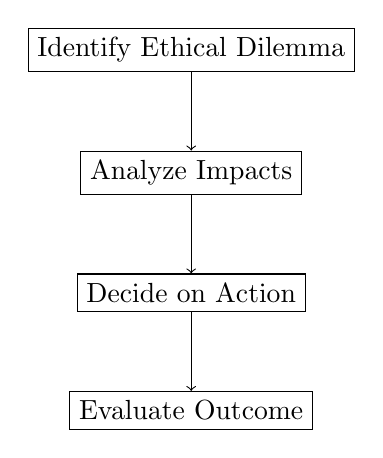
\begin{tikzpicture}
            \node (a) [draw, rectangle] {Identify Ethical Dilemma};
            \node (b) [draw, rectangle, below=of a] {Analyze Impacts};
            \node (c) [draw, rectangle, below=of b] {Decide on Action};
            \node (d) [draw, rectangle, below=of c] {Evaluate Outcome};

            \draw[->] (a) -- (b);
            \draw[->] (b) -- (c);
            \draw[->] (c) -- (d);
        \end{tikzpicture}
    \end{center}
\end{frame}

\begin{frame}[fragile]
    \frametitle{Conclusion}
    As DRL systems evolve, addressing ethical issues is critical for building trust and ensuring responsible use. The goal is to create systems that not only perform well but also align with societal values and ethical standards.
\end{frame}

\begin{frame}[fragile]
  \frametitle{Conclusion and Future Directions - Part 1}
  \begin{block}{Summary of Deep Reinforcement Learning}
    \begin{itemize}
      \item \textbf{Deep Reinforcement Learning (DRL)} combines RL principles with deep learning techniques.
      \item Key components discussed:
        \begin{enumerate}
          \item \textbf{Foundational Concepts:} Learning through interaction with the environment and using deep neural networks to approximate functions.
          \item \textbf{Algorithms:} Importance of DQN, Policy Gradients, and Actor-Critic methods, showcasing enhanced learning.
          \item \textbf{Applications:} Diverse fields like gaming, robotics, finance, and automated systems exemplify DRL's effectiveness.
          \item \textbf{Ethical Considerations:} Addressing bias, safety, and transparency in DRL algorithms is crucial.
        \end{enumerate}
    \end{itemize}
  \end{block}
\end{frame}

\begin{frame}[fragile]
  \frametitle{Conclusion and Future Directions - Part 2}
  \begin{block}{Future Directions in Deep Reinforcement Learning}
    \begin{itemize}
      \item \textbf{Multi-Agent Systems:} Collaboration and competition among agents can enhance learning. 
        \begin{itemize}
          \item Example: Autonomous vehicles interacting in driving simulations.
        \end{itemize}
      \item \textbf{Transfer Learning and Generalization:} Agents learn from one domain to solve problems in another, minimizing retraining.
        \begin{itemize}
          \item Example: Using strategies from virtual environments in real-world applications.
        \end{itemize}
      \item \textbf{Integration with Other AI Modalities:} Merging DRL with NLP and computer vision creates versatile AI systems.
        \begin{itemize}
          \item Example: Robots that understand verbal commands while navigating.
        \end{itemize}
    \end{itemize}
  \end{block}
\end{frame}

\begin{frame}[fragile]
  \frametitle{Conclusion and Future Directions - Part 3}
  \begin{block}{Future Directions (Continued)}
    \begin{itemize}
      \item \textbf{Interpretability and Safety:} Enhancing model interpretability to ensure reliability and understandability, especially in critical areas like healthcare and finance.
      \item \textbf{Real-World Deployment:} Focus on efficiency and robustness to operate effectively in real environments.
        \begin{itemize}
          \item Example: Implementing DRL in smart grid management for energy optimization.
        \end{itemize}
    \end{itemize}
  \end{block}

  \begin{block}{Key Takeaways}
    \begin{itemize}
      \item DRL merges RL and deep learning, leading to advancements across sectors.
      \item Ethical considerations should guide DRL development.
      \item Future trends in DRL show immense potential for innovation.
    \end{itemize}
  \end{block}

  \begin{block}{Closing Remark}
    As we innovate within DRL, our dedication to ethics and application will shape its societal impact.
  \end{block}
\end{frame}


\end{document}